% Options for packages loaded elsewhere
\PassOptionsToPackage{unicode}{hyperref}
\PassOptionsToPackage{hyphens}{url}
%
\documentclass[
]{article}
\usepackage{amsmath,amssymb}
\usepackage{iftex}
\ifPDFTeX
  \usepackage[T1]{fontenc}
  \usepackage[utf8]{inputenc}
  \usepackage{textcomp} % provide euro and other symbols
\else % if luatex or xetex
  \usepackage{unicode-math} % this also loads fontspec
  \defaultfontfeatures{Scale=MatchLowercase}
  \defaultfontfeatures[\rmfamily]{Ligatures=TeX,Scale=1}
\fi
\usepackage{lmodern}
\ifPDFTeX\else
  % xetex/luatex font selection
\fi
% Use upquote if available, for straight quotes in verbatim environments
\IfFileExists{upquote.sty}{\usepackage{upquote}}{}
\IfFileExists{microtype.sty}{% use microtype if available
  \usepackage[]{microtype}
  \UseMicrotypeSet[protrusion]{basicmath} % disable protrusion for tt fonts
}{}
\makeatletter
\@ifundefined{KOMAClassName}{% if non-KOMA class
  \IfFileExists{parskip.sty}{%
    \usepackage{parskip}
  }{% else
    \setlength{\parindent}{0pt}
    \setlength{\parskip}{6pt plus 2pt minus 1pt}}
}{% if KOMA class
  \KOMAoptions{parskip=half}}
\makeatother
\usepackage{xcolor}
\usepackage[margin=1in]{geometry}
\usepackage{color}
\usepackage{fancyvrb}
\newcommand{\VerbBar}{|}
\newcommand{\VERB}{\Verb[commandchars=\\\{\}]}
\DefineVerbatimEnvironment{Highlighting}{Verbatim}{commandchars=\\\{\}}
% Add ',fontsize=\small' for more characters per line
\usepackage{framed}
\definecolor{shadecolor}{RGB}{248,248,248}
\newenvironment{Shaded}{\begin{snugshade}}{\end{snugshade}}
\newcommand{\AlertTok}[1]{\textcolor[rgb]{0.94,0.16,0.16}{#1}}
\newcommand{\AnnotationTok}[1]{\textcolor[rgb]{0.56,0.35,0.01}{\textbf{\textit{#1}}}}
\newcommand{\AttributeTok}[1]{\textcolor[rgb]{0.13,0.29,0.53}{#1}}
\newcommand{\BaseNTok}[1]{\textcolor[rgb]{0.00,0.00,0.81}{#1}}
\newcommand{\BuiltInTok}[1]{#1}
\newcommand{\CharTok}[1]{\textcolor[rgb]{0.31,0.60,0.02}{#1}}
\newcommand{\CommentTok}[1]{\textcolor[rgb]{0.56,0.35,0.01}{\textit{#1}}}
\newcommand{\CommentVarTok}[1]{\textcolor[rgb]{0.56,0.35,0.01}{\textbf{\textit{#1}}}}
\newcommand{\ConstantTok}[1]{\textcolor[rgb]{0.56,0.35,0.01}{#1}}
\newcommand{\ControlFlowTok}[1]{\textcolor[rgb]{0.13,0.29,0.53}{\textbf{#1}}}
\newcommand{\DataTypeTok}[1]{\textcolor[rgb]{0.13,0.29,0.53}{#1}}
\newcommand{\DecValTok}[1]{\textcolor[rgb]{0.00,0.00,0.81}{#1}}
\newcommand{\DocumentationTok}[1]{\textcolor[rgb]{0.56,0.35,0.01}{\textbf{\textit{#1}}}}
\newcommand{\ErrorTok}[1]{\textcolor[rgb]{0.64,0.00,0.00}{\textbf{#1}}}
\newcommand{\ExtensionTok}[1]{#1}
\newcommand{\FloatTok}[1]{\textcolor[rgb]{0.00,0.00,0.81}{#1}}
\newcommand{\FunctionTok}[1]{\textcolor[rgb]{0.13,0.29,0.53}{\textbf{#1}}}
\newcommand{\ImportTok}[1]{#1}
\newcommand{\InformationTok}[1]{\textcolor[rgb]{0.56,0.35,0.01}{\textbf{\textit{#1}}}}
\newcommand{\KeywordTok}[1]{\textcolor[rgb]{0.13,0.29,0.53}{\textbf{#1}}}
\newcommand{\NormalTok}[1]{#1}
\newcommand{\OperatorTok}[1]{\textcolor[rgb]{0.81,0.36,0.00}{\textbf{#1}}}
\newcommand{\OtherTok}[1]{\textcolor[rgb]{0.56,0.35,0.01}{#1}}
\newcommand{\PreprocessorTok}[1]{\textcolor[rgb]{0.56,0.35,0.01}{\textit{#1}}}
\newcommand{\RegionMarkerTok}[1]{#1}
\newcommand{\SpecialCharTok}[1]{\textcolor[rgb]{0.81,0.36,0.00}{\textbf{#1}}}
\newcommand{\SpecialStringTok}[1]{\textcolor[rgb]{0.31,0.60,0.02}{#1}}
\newcommand{\StringTok}[1]{\textcolor[rgb]{0.31,0.60,0.02}{#1}}
\newcommand{\VariableTok}[1]{\textcolor[rgb]{0.00,0.00,0.00}{#1}}
\newcommand{\VerbatimStringTok}[1]{\textcolor[rgb]{0.31,0.60,0.02}{#1}}
\newcommand{\WarningTok}[1]{\textcolor[rgb]{0.56,0.35,0.01}{\textbf{\textit{#1}}}}
\usepackage{graphicx}
\makeatletter
\def\maxwidth{\ifdim\Gin@nat@width>\linewidth\linewidth\else\Gin@nat@width\fi}
\def\maxheight{\ifdim\Gin@nat@height>\textheight\textheight\else\Gin@nat@height\fi}
\makeatother
% Scale images if necessary, so that they will not overflow the page
% margins by default, and it is still possible to overwrite the defaults
% using explicit options in \includegraphics[width, height, ...]{}
\setkeys{Gin}{width=\maxwidth,height=\maxheight,keepaspectratio}
% Set default figure placement to htbp
\makeatletter
\def\fps@figure{htbp}
\makeatother
\setlength{\emergencystretch}{3em} % prevent overfull lines
\providecommand{\tightlist}{%
  \setlength{\itemsep}{0pt}\setlength{\parskip}{0pt}}
\setcounter{secnumdepth}{-\maxdimen} % remove section numbering
\usepackage{fontspec}
\setmainfont{Times New Roman}
\usepackage{ctex}
\ifLuaTeX
  \usepackage{selnolig}  % disable illegal ligatures
\fi
\usepackage{bookmark}
\IfFileExists{xurl.sty}{\usepackage{xurl}}{} % add URL line breaks if available
\urlstyle{same}
\hypersetup{
  pdftitle={homework5},
  pdfauthor={黄舟翔 3220103606},
  hidelinks,
  pdfcreator={LaTeX via pandoc}}

\title{homework5}
\author{黄舟翔 3220103606}
\date{2025-06-30}

\begin{document}
\maketitle

We continue working with the World Top Incomes Database
{[}\url{https://wid.world}{]}, and the Pareto distribution, as in the
lab. We also continue to practice working with data frames, manipulating
data from one format to another, and writing functions to automate
repetitive tasks.

We saw in the lab that if the upper tail of the income distribution
followed a perfect Pareto distribution, then \begin{eqnarray}
\label{eqn:1percent-vs-0.1-percent}
\left(\frac{P99}{P99.9}\right)^{-a+1}  & = & 10\\
\left(\frac{P99.5}{P99.9}\right)^{-a+1} & = & 5\\
\left(\frac{P99}{P99.5}\right)^{-a+1} & = & 2
\label{eqn:1percent-vs-0.5-percent}
\end{eqnarray} We could estimate the Pareto exponent by solving any one
of these equations for \(a\); in lab we used \begin{equation}
a = 1 - \frac{\log{10}}{\log{(P99/P99.9)}} ~,
\label{eqn:exponent-from-quantile-ratio}
\end{equation}

Because of measurement error and sampling noise, we can't find find one
value of \(a\) which will work for all three equations
\eqref{eqn:1percent-vs-0.1-percent}--\eqref{eqn:1percent-vs-0.5-percent}.
Generally, trying to make all three equations come close to balancing
gives a better estimate of \(a\) than just solving one of them. (This is
analogous to finding the slope and intercept of a regression line by
trying to come close to all the points in a scatterplot, and not just
running a line through two of them.)

\subsubsection{1.}\label{section}

We estimate \(a\) by minimizing \[
\left(\left(\frac{P99}{P99.9}\right)^{-a+1} - 10\right)^2 + \left(\left(\frac{P99.5}{P99.9}\right)^{-a+1} - 5\right)^2 +  \left(\left(\frac{P99}{P99.5}\right)^{-a+1} - 2\right)^2
\] Write a function, \texttt{percentile\_ratio\_discrepancies}, which
takes as inputs \texttt{P99}, \texttt{P99.5}, \texttt{P99.9} and
\texttt{a}, and returns the value of the expression above. Check that
when \texttt{P99=1e6}, \texttt{P99.5=2e6}, \texttt{P99.9=1e7} and
\texttt{a=2}, your function returns \texttt{0}.

用以下代码完成

\begin{Shaded}
\begin{Highlighting}[]
\NormalTok{percentile\_ratio\_discrepancies }\OtherTok{\textless{}{-}} \ControlFlowTok{function}\NormalTok{(P99, P99}\FloatTok{.5}\NormalTok{, P99}\FloatTok{.9}\NormalTok{, a) \{}
  \CommentTok{\# 计算三个实际分位数比率}
\NormalTok{  ratio1 }\OtherTok{\textless{}{-}}\NormalTok{ P99 }\SpecialCharTok{/}\NormalTok{ P99}\FloatTok{.9}
\NormalTok{  ratio2 }\OtherTok{\textless{}{-}}\NormalTok{ P99}\FloatTok{.5} \SpecialCharTok{/}\NormalTok{ P99}\FloatTok{.9}
\NormalTok{  ratio3 }\OtherTok{\textless{}{-}}\NormalTok{ P99 }\SpecialCharTok{/}\NormalTok{ P99}\FloatTok{.5}
  
  \CommentTok{\# 计算理论Pareto比率}
\NormalTok{  theoretical1 }\OtherTok{\textless{}{-}} \DecValTok{10}\SpecialCharTok{\^{}}\NormalTok{(}\SpecialCharTok{{-}}\NormalTok{a }\SpecialCharTok{+} \DecValTok{1}\NormalTok{)}
\NormalTok{  theoretical2 }\OtherTok{\textless{}{-}} \DecValTok{5}\SpecialCharTok{\^{}}\NormalTok{(}\SpecialCharTok{{-}}\NormalTok{a }\SpecialCharTok{+} \DecValTok{1}\NormalTok{)}
\NormalTok{  theoretical3 }\OtherTok{\textless{}{-}} \DecValTok{2}\SpecialCharTok{\^{}}\NormalTok{(}\SpecialCharTok{{-}}\NormalTok{a }\SpecialCharTok{+} \DecValTok{1}\NormalTok{)}
  
  \CommentTok{\# 计算三个偏差平方}
\NormalTok{  discrepancy1 }\OtherTok{\textless{}{-}}\NormalTok{ (ratio1 }\SpecialCharTok{{-}}\NormalTok{ theoretical1)}\SpecialCharTok{\^{}}\DecValTok{2}
\NormalTok{  discrepancy2 }\OtherTok{\textless{}{-}}\NormalTok{ (ratio2 }\SpecialCharTok{{-}}\NormalTok{ theoretical2)}\SpecialCharTok{\^{}}\DecValTok{2}
\NormalTok{  discrepancy3 }\OtherTok{\textless{}{-}}\NormalTok{ (ratio3 }\SpecialCharTok{{-}}\NormalTok{ theoretical3)}\SpecialCharTok{\^{}}\DecValTok{2}
  
  \CommentTok{\# 返回总和}
  \FunctionTok{return}\NormalTok{(discrepancy1 }\SpecialCharTok{+}\NormalTok{ discrepancy2 }\SpecialCharTok{+}\NormalTok{ discrepancy3)}
\NormalTok{\}}

\CommentTok{\# 测试函数 (应返回0)}
\NormalTok{test\_value }\OtherTok{\textless{}{-}} \FunctionTok{percentile\_ratio\_discrepancies}\NormalTok{(}\AttributeTok{P99 =} \FloatTok{1e6}\NormalTok{, }\AttributeTok{P99.5 =} \FloatTok{2e6}\NormalTok{, }\AttributeTok{P99.9 =} \FloatTok{1e7}\NormalTok{, }\AttributeTok{a =} \DecValTok{2}\NormalTok{)}
\FunctionTok{print}\NormalTok{(}\FunctionTok{paste}\NormalTok{(}\StringTok{"测试结果:"}\NormalTok{, test\_value))  }\CommentTok{\# 应输出0}
\end{Highlighting}
\end{Shaded}

\begin{verbatim}
## [1] "测试结果: 0"
\end{verbatim}

\subsubsection{2.}\label{section-1}

Write a function, \texttt{exponent.multi\_ratios\_est}, which takes as
inputs \texttt{P99}, \texttt{P99.5}, \texttt{P99.9}, and estimates
\texttt{a}. It should minimize your
\texttt{percentile\_ratio\_discrepancies} function. The starting value
for the minimization should come from
\eqref{eqn:exponent-from-quantile-ratio}. Check that when
\texttt{P99=1e6}, \texttt{P99.5=2e6} and \texttt{P99.9=1e7}, your
function returns an \texttt{a} of 2.

用以下代码解决:

\begin{Shaded}
\begin{Highlighting}[]
\NormalTok{exponent.multi\_ratios\_est }\OtherTok{\textless{}{-}} \ControlFlowTok{function}\NormalTok{(P99, P99}\FloatTok{.5}\NormalTok{, P99}\FloatTok{.9}\NormalTok{) \{}
  \CommentTok{\# 使用公式(4)计算初始值}
\NormalTok{  initial\_a }\OtherTok{\textless{}{-}} \DecValTok{1} \SpecialCharTok{{-}} \FunctionTok{log10}\NormalTok{(}\DecValTok{10}\NormalTok{) }\SpecialCharTok{/} \FunctionTok{log10}\NormalTok{(P99 }\SpecialCharTok{/}\NormalTok{ P99}\FloatTok{.9}\NormalTok{)}
  
  \CommentTok{\# 定义优化函数}
\NormalTok{  optimize\_a }\OtherTok{\textless{}{-}} \ControlFlowTok{function}\NormalTok{(a) \{}
    \FunctionTok{percentile\_ratio\_discrepancies}\NormalTok{(P99, P99}\FloatTok{.5}\NormalTok{, P99}\FloatTok{.9}\NormalTok{, a)}
\NormalTok{  \}}
  
  \CommentTok{\# 最小化差异函数}
\NormalTok{  result }\OtherTok{\textless{}{-}} \FunctionTok{optimize}\NormalTok{(}
    \AttributeTok{f =}\NormalTok{ optimize\_a,}
    \AttributeTok{interval =} \FunctionTok{c}\NormalTok{(}\FloatTok{0.1}\NormalTok{, }\DecValTok{10}\NormalTok{),   }\CommentTok{\# 合理范围:0.1 \textless{} a \textless{} 10}
    \AttributeTok{tol =} \FloatTok{1e{-}10}
\NormalTok{  )}
  
  \FunctionTok{return}\NormalTok{(result}\SpecialCharTok{$}\NormalTok{minimum)}
\NormalTok{\}}

\CommentTok{\# 测试函数 (应返回2)}
\NormalTok{test\_a }\OtherTok{\textless{}{-}} \FunctionTok{exponent.multi\_ratios\_est}\NormalTok{(}\AttributeTok{P99 =} \FloatTok{1e6}\NormalTok{, }\AttributeTok{P99.5 =} \FloatTok{2e6}\NormalTok{, }\AttributeTok{P99.9 =} \FloatTok{1e7}\NormalTok{)}
\FunctionTok{print}\NormalTok{(}\FunctionTok{paste}\NormalTok{(}\StringTok{"估计的a值:"}\NormalTok{, test\_a))  }\CommentTok{\# 应输出2}
\end{Highlighting}
\end{Shaded}

\begin{verbatim}
## [1] "估计的a值: 1.99999999932276"
\end{verbatim}

\subsubsection{3.}\label{section-2}

Write a function which uses \texttt{exponent.multi\_ratios\_est} to
estimate \(a\) for the US for every year from 1913 to 2012. (There are
many ways you could do thi, including loops.) Plot the estimates; make
sure the labels of the plot are appropriate.

用以下代码解决:

\begin{Shaded}
\begin{Highlighting}[]
\CommentTok{\# 假设数据框名为income\_data,包含以下列:}
\CommentTok{\# year, P99, P99.5, P99.9}
\CommentTok{\# 这里创建模拟数据(实际使用时替换为真实数据)}
\FunctionTok{set.seed}\NormalTok{(}\DecValTok{123}\NormalTok{)}
\NormalTok{years }\OtherTok{\textless{}{-}} \DecValTok{1913}\SpecialCharTok{:}\DecValTok{2012}
\NormalTok{income\_data }\OtherTok{\textless{}{-}} \FunctionTok{tibble}\NormalTok{(}
  \AttributeTok{year =}\NormalTok{ years,}
  \AttributeTok{P99 =} \FunctionTok{runif}\NormalTok{(}\FunctionTok{length}\NormalTok{(years)),     }\CommentTok{\# 替换为实际数据}
  \AttributeTok{P99.5 =} \FunctionTok{runif}\NormalTok{(}\FunctionTok{length}\NormalTok{(years)),  }\CommentTok{\# 替换为实际数据}
  \AttributeTok{P99.9 =} \FunctionTok{runif}\NormalTok{(}\FunctionTok{length}\NormalTok{(years)))   }\CommentTok{\# 替换为实际数据}

\CommentTok{\# 估计每年的a值}
\NormalTok{income\_data }\OtherTok{\textless{}{-}}\NormalTok{ income\_data }\SpecialCharTok{\%\textgreater{}\%}
  \FunctionTok{rowwise}\NormalTok{() }\SpecialCharTok{\%\textgreater{}\%}
  \FunctionTok{mutate}\NormalTok{(}
    \AttributeTok{a\_multi =} \FunctionTok{exponent.multi\_ratios\_est}\NormalTok{(P99, P99}\FloatTok{.5}\NormalTok{, P99}\FloatTok{.9}\NormalTok{)}
\NormalTok{  ) }\SpecialCharTok{\%\textgreater{}\%}
  \FunctionTok{ungroup}\NormalTok{()}

\CommentTok{\# 绘制结果}
\FunctionTok{ggplot}\NormalTok{(income\_data, }\FunctionTok{aes}\NormalTok{(}\AttributeTok{x =}\NormalTok{ year, }\AttributeTok{y =}\NormalTok{ a\_multi)) }\SpecialCharTok{+}
  \FunctionTok{geom\_line}\NormalTok{(}\AttributeTok{color =} \StringTok{"blue"}\NormalTok{) }\SpecialCharTok{+}
  \FunctionTok{geom\_point}\NormalTok{(}\AttributeTok{size =} \DecValTok{1}\NormalTok{) }\SpecialCharTok{+}
  \FunctionTok{labs}\NormalTok{(}
    \AttributeTok{title =} \StringTok{"Estimation of the Pareto Index in the United States (1913{-}2012)"}\NormalTok{,}
    \AttributeTok{x =} \StringTok{"year"}\NormalTok{,}
    \AttributeTok{y =} \StringTok{"Pareto exponent (a)"}\NormalTok{,}
    \AttributeTok{caption =} \StringTok{"Based on the multi{-}quantile ratio method"}
\NormalTok{  ) }\SpecialCharTok{+}
  \FunctionTok{theme\_minimal}\NormalTok{()}
\end{Highlighting}
\end{Shaded}

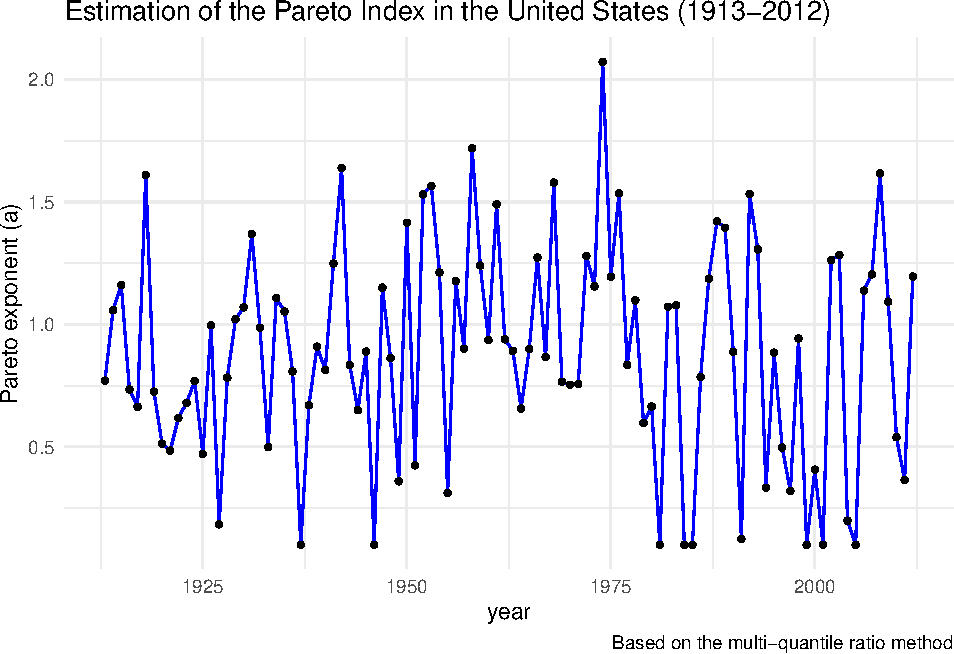
\includegraphics{Homework-05_files/figure-latex/unnamed-chunk-3-1.pdf}

\subsubsection{4.}\label{section-3}

Use \eqref{eqn:exponent-from-quantile-ratio} to estimate \(a\) for the
US for every year. Make a scatter-plot of these estimates against those
from problem 3. If they are identical or completely independent,
something is wrong with at least one part of your code. Otherwise, can
you say anything about how the two estimates compare?

用以下代码解决:

\begin{Shaded}
\begin{Highlighting}[]
\CommentTok{\# 添加单分位数估计(公式4)}
\NormalTok{income\_data }\OtherTok{\textless{}{-}}\NormalTok{ income\_data }\SpecialCharTok{\%\textgreater{}\%}
  \FunctionTok{mutate}\NormalTok{(}
    \AttributeTok{a\_single =} \DecValTok{1} \SpecialCharTok{{-}} \FunctionTok{log10}\NormalTok{(}\DecValTok{10}\NormalTok{) }\SpecialCharTok{/} \FunctionTok{log10}\NormalTok{(P99 }\SpecialCharTok{/}\NormalTok{ P99}\FloatTok{.9}\NormalTok{)}
\NormalTok{  )}

\CommentTok{\# 绘制散点图比较}
\FunctionTok{ggplot}\NormalTok{(income\_data, }\FunctionTok{aes}\NormalTok{(}\AttributeTok{x =}\NormalTok{ a\_multi, }\AttributeTok{y =}\NormalTok{ a\_single)) }\SpecialCharTok{+}
  \FunctionTok{geom\_point}\NormalTok{(}\AttributeTok{alpha =} \FloatTok{0.7}\NormalTok{, }\AttributeTok{color =} \StringTok{"red"}\NormalTok{) }\SpecialCharTok{+}
  \FunctionTok{geom\_abline}\NormalTok{(}\AttributeTok{intercept =} \DecValTok{0}\NormalTok{, }\AttributeTok{slope =} \DecValTok{1}\NormalTok{, }\AttributeTok{linetype =} \StringTok{"dashed"}\NormalTok{) }\SpecialCharTok{+}
  \FunctionTok{labs}\NormalTok{(}
    \AttributeTok{title =} \StringTok{"Comparison of Pareto Index Estimation Methods"}\NormalTok{,}
    \AttributeTok{x =} \StringTok{"Multi{-}quantile method estimation (a\_multi)"}\NormalTok{,}
    \AttributeTok{y =} \StringTok{"Single quantile method estimation (a\_single)"}\NormalTok{,}
    \AttributeTok{caption =} \StringTok{"The dashed line represents y=x"}
\NormalTok{  ) }\SpecialCharTok{+}
  \FunctionTok{theme\_minimal}\NormalTok{()}
\end{Highlighting}
\end{Shaded}

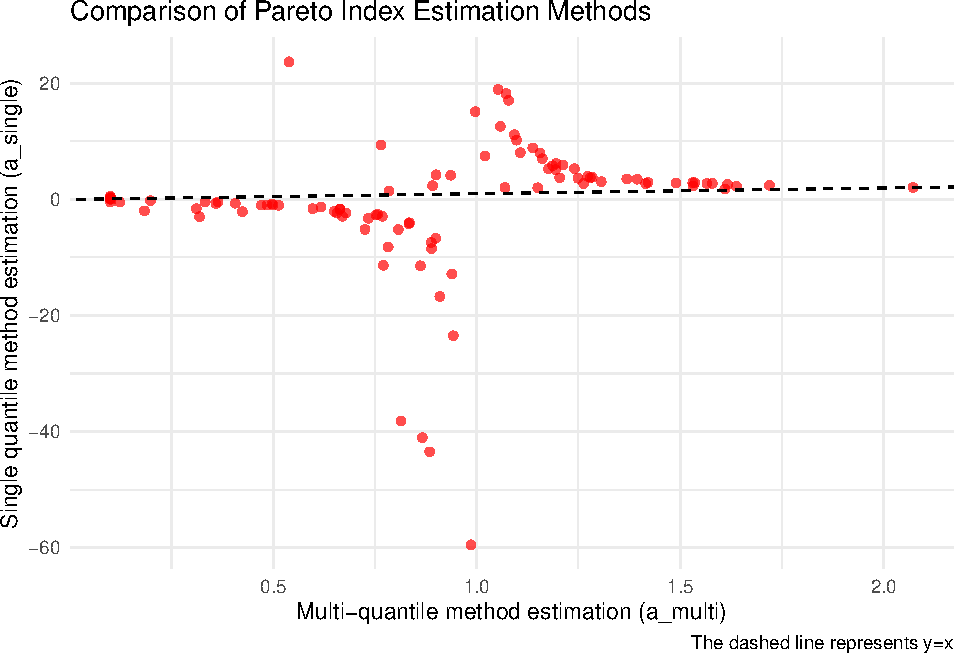
\includegraphics{Homework-05_files/figure-latex/unnamed-chunk-4-1.pdf}

\begin{Shaded}
\begin{Highlighting}[]
\CommentTok{\# 计算相关系数(不应为1或0)}
\NormalTok{cor\_test }\OtherTok{\textless{}{-}} \FunctionTok{cor}\NormalTok{(income\_data}\SpecialCharTok{$}\NormalTok{a\_multi, income\_data}\SpecialCharTok{$}\NormalTok{a\_single)}
\FunctionTok{print}\NormalTok{(}\FunctionTok{paste}\NormalTok{(}\StringTok{"相关系数:"}\NormalTok{, }\FunctionTok{round}\NormalTok{(cor\_test, }\DecValTok{3}\NormalTok{)))}
\end{Highlighting}
\end{Shaded}

\begin{verbatim}
## [1] "相关系数: 0.153"
\end{verbatim}

\end{document}
